\documentclass{article}
\usepackage{graphicx}
\usepackage[margin=1.5cm]{geometry}
\usepackage{amsmath}

\begin{document}
\twocolumn

\title{Monday Warm Up: Unit 5: Momentum II}
\author{Prof. Jordan C. Hanson}

\maketitle

\section{Memory Bank}

\begin{itemize}
\item $\vec{p} = m\vec{v}$ ... Definition of momentum.
\item $\vec{p}_{\rm total} = \vec{p}_1 + \vec{p}_2$ ... Total momentum.
\item $\vec{p}_{\rm total,i} = \vec{p}_{\rm total,f}$ ... Momentum is conserved.
\item $\vec{F}_{\rm Net} = -\frac{d\vec{p}}{dt}$ ... Force and momentum
\end{itemize}

\section{Momentum}

\begin{enumerate}
\item What is the momentum (as a function of time) of a 5.0 kg particle moving with a velocity $\vec{v}(t)=(2.0\hat{i}+4.0t\hat{j})$ m s$^{-1}$? (a) What is the acceleration of this particle? (b) What is the net force acting on this particle? \\ \vspace{3cm}
\item Ernest Rutherford (the first New Zealander to be awarded the Nobel Prize in Chemistry) demonstrated that nuclei were very small and dense by scattering helium-4 nuclei from gold-197 nuclei. The energy of the incoming helium nucleus was $8.00\times 10^{−13}$ J, and the masses of the helium and gold nuclei were $6.68\times 10^{−27}$ kg and $3.29\times 10^{−25}$ kg, respectively (note that their mass ratio is 4 to 197). See Fig. \ref{fig:1}.  (a) If a helium nucleus scatters to an angle of 120° during an elastic collision with a gold nucleus, calculate the final speed of the helium nucleus and the final velocity (magnitude and direction) of the gold nucleus.  (b) What is the final kinetic energy of the helium nucleus? \\ \vspace{5cm}
\item A 200-kg rocket in deep space moves with a velocity of $121\hat{i}+38.0\hat{j}$ m s$^{-1}$. Suddenly, it explodes into three pieces, with the first (78 kg) moving at $−321\hat{i}+228\hat{j}$ m s$^{-1}$ and the second (56 kg) moving at $16.0\hat{i} - 88.0\hat{j}$ m s$^{-1}$. Find the velocity of the third piece.
\end{enumerate}

\begin{figure}
\centering
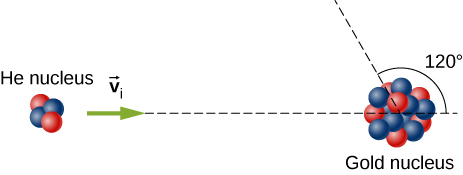
\includegraphics[width=0.4\textwidth]{figures/nuclei.jpeg}
\caption{\label{fig:1} An alpha particle (helium nucleus) interacting with a gold nucleus within an atom.}
\end{figure}

\end{document}
